% ============================================================
%  KUIS 3 — MATEMATIKA (MAE)  T.P. 2026/2027
%  Tema: "National Card Strategy Championship (NCSC)"
%  Bentuk: 1-5 PG Kompleks (Benar/Salah); 6-9 Uraian; 10 Rekomendasi;
%          11-12 BONUS
%  Materi inti: Bab 6 Statistika (6.1-6.5), Bab 7 Peluang (7.1-7.5)
%  Prinsip: "progressive dossier" -> Berkas A..D terbuka bertahap.
%  Data sinkron: rekap skor 40 peserta (x=25), set remi standar 52 kartu.
%  Kompilasi: pdfLaTeX (gambar berada di folder yang sama)
% ============================================================

\documentclass[11pt]{article}

% ===================== PACKAGES =====================
\usepackage[utf8]{inputenc}
\usepackage[T1]{fontenc}
\usepackage[bahasa]{babel}
\usepackage[a4paper,margin=2.5cm,top=2.8cm]{geometry}
\usepackage{amsmath,amssymb}
\usepackage{graphicx}
\usepackage{tikz}
\usetikzlibrary{arrows.meta}
\usepackage{array}
\usepackage{enumitem}
\usepackage{multicol}
\usepackage{xcolor}
\usepackage[most]{tcolorbox}
\usepackage{fancyhdr}
\usepackage{booktabs}
\usepackage{icomma}

% ===================== HEADER & FOOTER =====================
\pagestyle{fancy}\fancyhf{}
\lhead{\small KUIS 3: Matematika (MAE)}
\rhead{\small T.P. 2026/2027}
\cfoot{\small\thepage}
\renewcommand{\headrulewidth}{0.4pt}

% ===================== KOTAK SOAL =====================
\newtcolorbox{soal}[1]{
  breakable,
  colback=white,
  colframe=black,
  colbacktitle=black,
  coltitle=white,
  fonttitle=\bfseries\sffamily,
  title={Nomor #1},
  boxrule=0.8pt, arc=0pt,
  left=3mm, right=3mm, top=2mm, bottom=2mm}

% ===================== LABEL BERKAS DATA =====================
\newtcolorbox{berkas}[1]{
  colback=teal!5, colframe=teal!55!black, boxrule=0.6pt, arc=1pt,
  left=3mm,right=3mm,top=1.5mm,bottom=1.5mm,
  fonttitle=\bfseries\sffamily\color{white}, coltitle=white,
  colbacktitle=teal!55!black, title={#1}}

% ===================== PILIHAN GANDA KOMPLEKS (Benar/Salah) =====================
\newenvironment{bstabel}{%
  \par\smallskip\begin{center}\renewcommand{\arraystretch}{1.35}%
  \begin{tabular}{@{}p{0.72\textwidth}>{\centering\arraybackslash}m{1.5cm}>{\centering\arraybackslash}m{1.5cm}@{}}
  \toprule
  \textbf{Pernyataan} & \textbf{Benar} & \textbf{Salah}\\\midrule}%
  {\bottomrule\end{tabular}\end{center}}
\newcommand{\bs}[1]{#1 & $\square$ & $\square$\\[1pt]}

% ===================== SUB-SOAL URAIAN (a, b, c, ...) =====================
\newenvironment{subsoal}{%
  \begin{enumerate}[label=\textbf{(\alph*)},leftmargin=1.8em,itemsep=5pt,topsep=3pt]}%
  {\end{enumerate}}

% ===================== GAMBAR =====================
\newcommand{\gambar}[2][0.6\textwidth]{%
  \begin{center}\includegraphics[width=#1]{#2}\end{center}}

\linespread{1.05}

% ===================================================================
%                         ISI DOKUMEN
% ===================================================================
\begin{document}
\thispagestyle{empty}

% ===================== COVER + PETUNJUK (satu halaman) =====================

\begin{center}
  \fbox{\parbox{0.45\textwidth}{\centering\bfseries\large LEMBAR SOAL}}
\end{center}
\vspace{0.3cm}

\begin{center}
  {\LARGE\bfseries KUIS 3: MATEMATIKA (MAE)}\\[0.3em]
  {\large\itshape Studi Kasus \textit{National Card Strategy Championship}}
\end{center}
\vspace{0.3cm}

\begin{center}
  \begin{tabular}{@{\hspace{2cm}}l@{\hspace{0.4cm}:\hspace{0.4cm}}l}
    Jenjang      & SMA / Madrasah Aliyah \\[0.3em]
    Hari/Tanggal & [\underline{\hspace{4cm}}] \\[0.3em]
    Waktu        & 120 menit \\[0.3em]
    Paket Soal   & -- \\
  \end{tabular}
\end{center}

\vspace{0.25cm}
\noindent\rule{\linewidth}{0.6pt}
\vspace{0.15cm}

\noindent\textbf{\underline{PETUNJUK UMUM}}
\begin{enumerate}[leftmargin=*,itemsep=2.5pt,topsep=2pt]
  \item Anda \textbf{tidak} diperbolehkan menggunakan sumber eksternal, termasuk
        internet dan \textit{large language model} (ChatGPT, Claude, Gemini, dan
        sebagainya). Kerjakan sendiri, karena kuis ini dibuat untuk
        \textbf{mengukur} tingkat kepahaman Anda.
  \item Soal terdiri atas \textbf{10 butir wajib (Nomor 1--10)} dan \textbf{2 butir
        bonus (Nomor 11--12)}, dan saling \textbf{berkolaborasi}: hasil pada nomor
        awal sering dipakai kembali (khususnya pada Nomor 10). Kerjakan
        \textbf{berurutan}.
  \item Kuis ini memakai \textbf{\textit{progressive dossier}}: berkas data
        turnamen terbuka bertahap dalam \textbf{Berkas A--D}. \textbf{Banyak data
        dibaca langsung dari berkas (tabel/gambar)}: amati tabel frekuensi, diagram
        pencar, dan susunan set kartu remi.
  \item \textbf{Bagian A (Nomor 1--5)} pilihan ganda kompleks (centang
        \textbf{Benar}/\textbf{Salah} tiap pernyataan). \textbf{Bagian B (Nomor
        6--9)} uraian bercabang; proses ikut dinilai. \textbf{Bagian C (Nomor 10)}
        sintesis lintas-bab (Bab 6--7): menghitung \emph{sekaligus} menyimpulkan
        seperti seorang analis.
  \item \textbf{Bagian D (Nomor 11--12): BONUS.} Benar menambah poin; salah/kosong
        tidak mengurangi. Kerjakan hanya jika Nomor 1--10 selesai.
  \item Materi inti: \textbf{Statistika} (Bab 6: distribusi frekuensi, pemusatan,
        letak, penyebaran, diagram pencar) dan \textbf{Peluang} (Bab 7: pencacahan,
        ruang sampel, peluang kejadian, frekuensi harapan, kejadian majemuk).
  \item Diperbolehkan memakai \textbf{kalkulator saintifik (non-programmable)}.
        \textbf{Nilai bantu:}\\[0.2em]
        \small
        $52\times51\times50=132.600$;\ \ $\binom{52}{3}=22.100$;\ \
        $\binom{52}{5}=2.598.960$;\ \ $\binom{13}{5}=1.287$;\ \
        $\binom{4}{2}=6$;\ \ $\binom{48}{3}=17.296$;\ \
        $1.300\div13=100$;\ \ $\sqrt{144{,}75}\approx12{,}03$.
  \item Isilah detail berikut.\\[0.3em]
        \textbf{Nama}\hspace{0.45cm};\enspace\underline{\hspace{8cm}}
\end{enumerate}

\vspace{0.2cm}
\noindent\textit{Dengan menandatangani kolom di bawah ini, saya menyatakan telah
membaca, memahami, dan menyetujui seluruh peraturan di atas.}

\vspace{0.25cm}
\noindent\fbox{\parbox{5cm}{\vspace{1.3cm}\centering\small Tanda Tangan Peserta\vspace{0.25cm}}}

\clearpage

% ===================================================================
%                 JUDUL + NARASI (data menyatu di cerita)
% ===================================================================

\begin{center}
  {\Large\bfseries \textit{National Card Strategy Championship}: Panggung Sang Analis}
\end{center}
\vspace{0.3cm}

\begin{center}
  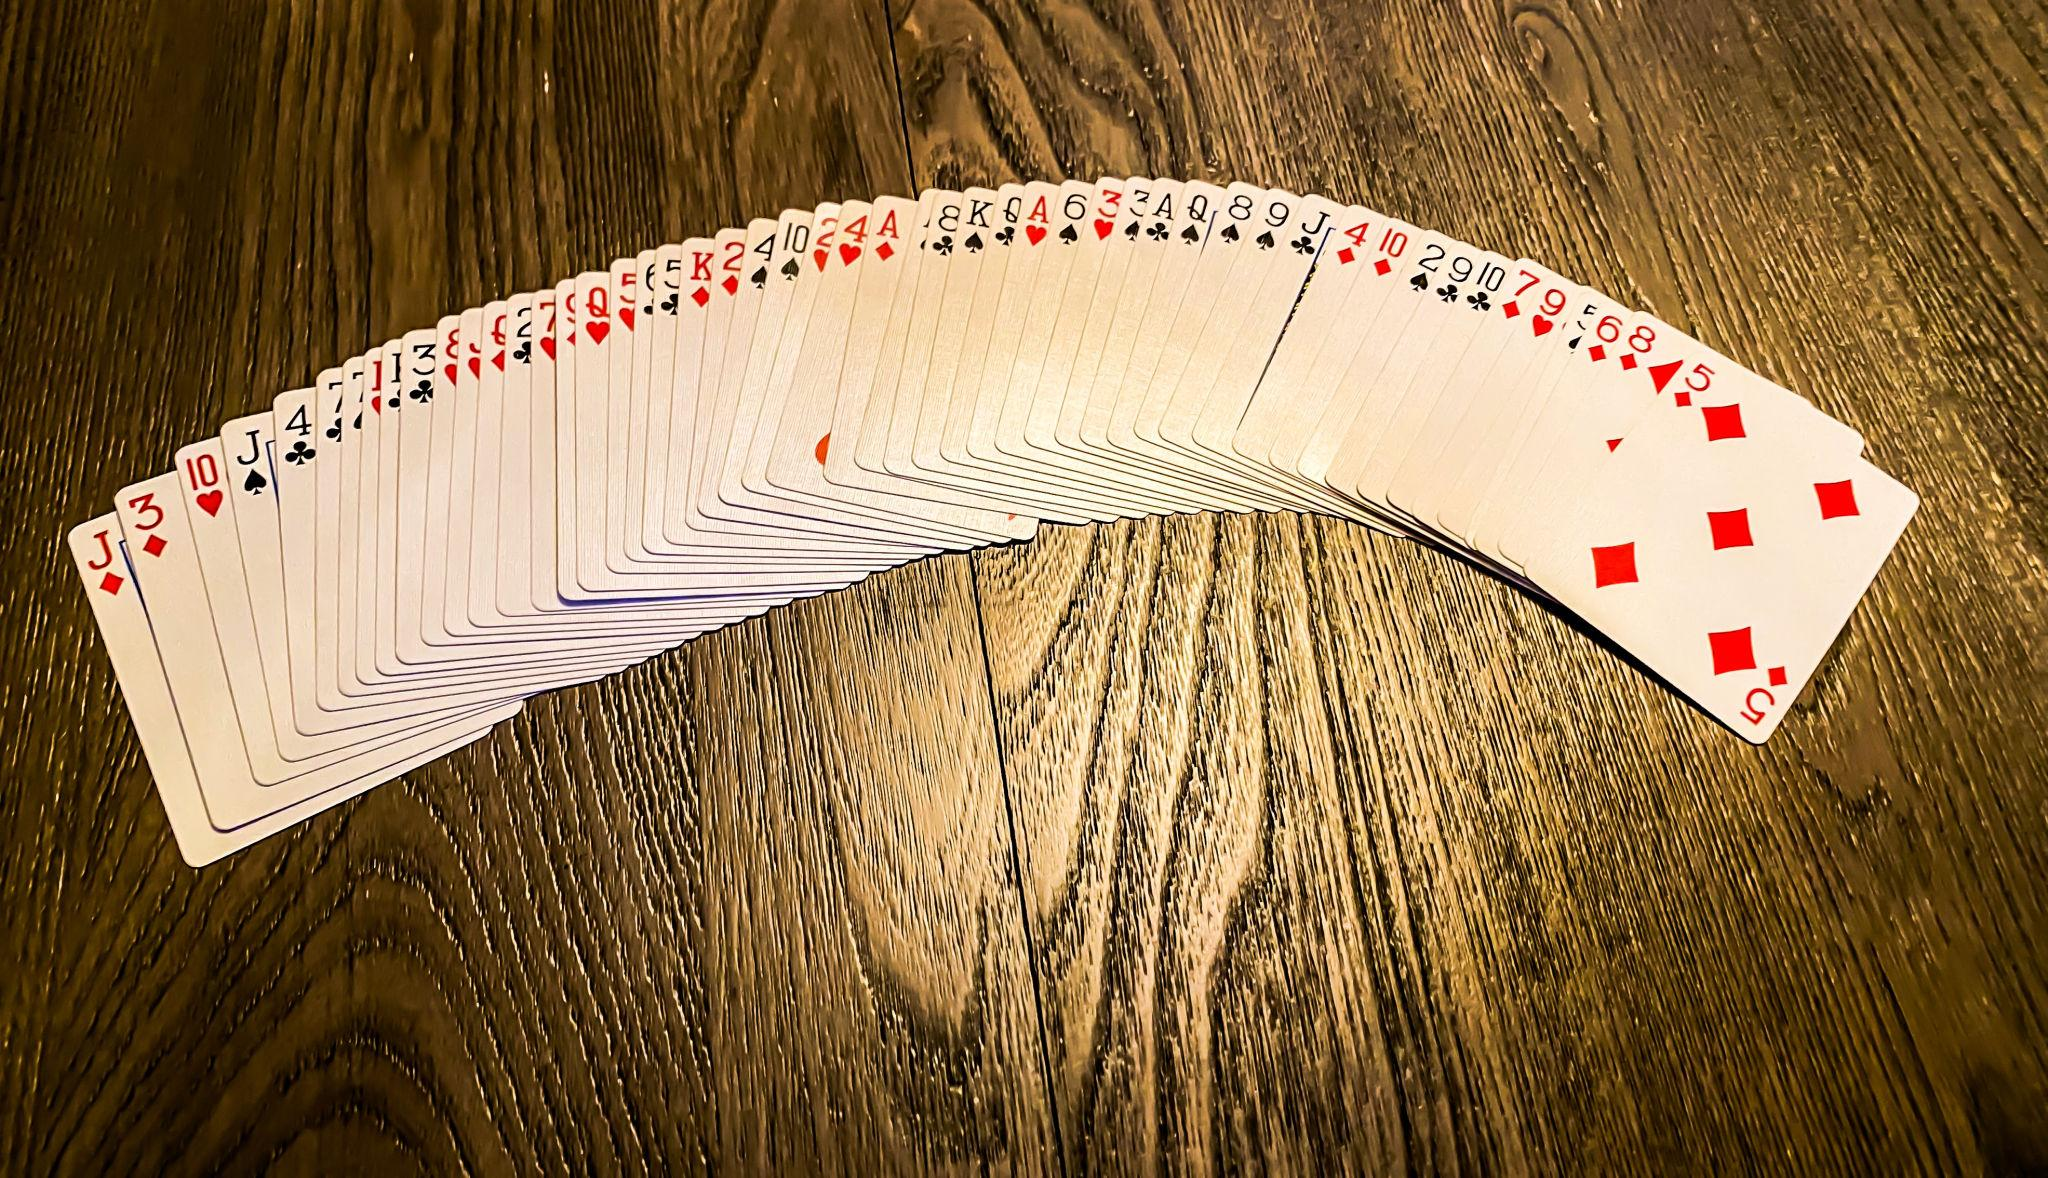
\includegraphics[width=0.85\textwidth]{remi-deck.jpg}\\[3pt]
  {\small\textit{Media pertandingan resmi NCSC: satu set kartu remi standar
  $52$ kartu ($4$ jenis/suit, masing-masing $13$ kartu; $26$ merah dan $26$
  hitam).}}
\end{center}
\vspace{0.15cm}

Setiap tahun, \textbf{\textit{National Card Strategy Championship} (NCSC)}
diselenggarakan untuk menguji kemampuan strategi, analisis, dan pengambilan
keputusan peserta melalui permainan kartu berbasis aturan. Ini \emph{bukan}
permainan taruhan, melainkan \textbf{kompetisi strategi} yang menggunakan
\textbf{satu set kartu remi standar berjumlah $52$ kartu} sebagai media
permainan. Seluruh pertandingan direkam secara digital.

\smallskip
Panitia mengumpulkan berbagai data: \textbf{skor akhir tiap peserta}, \textbf{lama
waktu berpikir pemain}, \textbf{jenis kartu yang muncul}, serta \textbf{distribusi
kombinasi kartu} selama turnamen. Sebagian rekap
dicatat pada lembar digital seperti berikut (contoh satu meja empat pemain
beserta \emph{poin minus} akhir dan sepuluh nomor \emph{kartu penentu kemenangan}
yang tercatat).

\begin{center}
  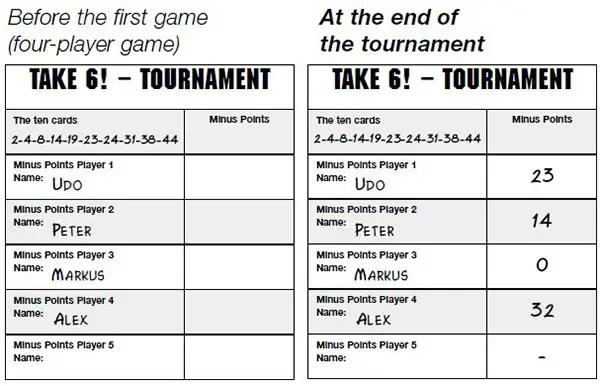
\includegraphics[width=0.7\textwidth]{tournament-score.jpg}\\[3pt]
  {\small\textit{Lembar rekap skor: makin kecil \emph{poin minus}, makin baik
  performa pemain. Empat pemain di atas memperoleh poin minus $23, 14, 0,$ dan
  $32$; sepuluh nomor kartu penentu: $2\text{-}4\text{-}8\text{-}14\text{-}19\text{-}23\text{-}24\text{-}31\text{-}38\text{-}44$.}}
\end{center}

\smallskip
Sebagai \textbf{\textit{Tournament Analyst}}, Anda diminta mengevaluasi hasil
turnamen dan memberikan rekomendasi kepada panitia \emph{berdasarkan analisis
matematika}. \textbf{Misi Anda:} menilai apakah sistem pertandingan telah
berlangsung secara \textbf{adil, seimbang, dan sesuai rancangan panitia}. Data
tidak diberikan sekaligus; ia terbuka bertahap dalam \textbf{Berkas A--D}, persis
seperti seorang analis membedah arsip pertandingan.

\smallskip
Alur analisis Anda menempuh tiga tahap: \textbf{(A) Analisis Statistik} atas hasil
pertandingan (Berkas A--B), \textbf{(B) Analisis Peluang} atas sistem pembagian
kartu (Berkas C), dan \textbf{(C) Sintesis \& Rekomendasi} yang memadukan
statistik dan peluang untuk menilai keadilan sistem. Selamat bertugas, Analis!

\vspace{0.3cm}
\noindent\rule{\linewidth}{0.6pt}
\vspace{0.1cm}

\noindent{\large\bfseries BAGIAN A: Analisis Statistik --- Pilihan Ganda Kompleks (Nomor 1--5)}\\[0.2em]
\small\emph{Panitia meminta Anda menyiapkan tiga keputusan dari data pertandingan:
\textbf{(i)} menguji klaim ``peserta rata-rata sudah bagus'' (Nomor 1--2),
\textbf{(ii)} menetapkan ambang \emph{gelar unggulan} dan \emph{zona evaluasi}
(Nomor 3), dan \textbf{(iii)} menilai ketat atau timpangnya persaingan (Nomor 4).
Baca berkas dengan teliti. Untuk tiap pernyataan, centang \textbf{Benar}/\textbf{Salah}.
Nomor 1--4 memakai Berkas A; Nomor 5 memakai Berkas B.}\normalsize

\bigskip

\begin{berkas}{Berkas A: Rekap Skor Akhir (Poin Minus) 40 Peserta Babak Final}
\small
Panitia merekap \textbf{skor akhir (poin minus)} dari \textbf{$40$ peserta}
babak final ke dalam tabel distribusi frekuensi berikut. Rekap ini akan dipakai
untuk menetapkan dua ambang: gelar \textbf{``peserta unggulan''} bagi $25\%$
peserta ber-poin minus \emph{terkecil}, dan \textbf{``zona evaluasi''} bagi $25\%$
peserta ber-poin minus \emph{terbesar}.
\begin{center}
\renewcommand{\arraystretch}{1.2}
\begin{tabular}{@{}c c@{\hspace{1.4cm}}c c@{}}
\toprule
\textbf{Interval Skor} & \textbf{Banyak Peserta ($f$)} &
\textbf{Interval Skor} & \textbf{Banyak Peserta ($f$)}\\
\midrule
$0$--$9$   & $4$  & $30$--$39$ & $8$\\
$10$--$19$ & $10$ & $40$--$49$ & $6$\\
$20$--$29$ & $12$ & \textbf{Jumlah} & $\mathbf{40}$\\
\bottomrule
\end{tabular}
\end{center}
\begin{center}
\begin{tikzpicture}[xscale=1.05,yscale=0.16]
\draw[->,gray] (0,0)--(5.8,0) node[right,font=\scriptsize]{interval};
\draw[->,gray] (0,0)--(0,14.5) node[above,font=\scriptsize]{$f$};
\foreach \f in {2,4,6,8,10,12} \draw[gray!40](0,\f)--(5.4,\f);
\foreach \i/\f/\lab in {0/4/{0-9}, 1/10/{10-19}, 2/12/{20-29}, 3/8/{30-39}, 4/6/{40-49}}{
  \fill[teal!30] (\i+0.15,0) rectangle (\i+0.85,\f);
  \draw[teal!55!black] (\i+0.15,0) rectangle (\i+0.85,\f);
  \node[below,font=\tiny] at (\i+0.5,0){\lab};
  \node[above,font=\tiny] at (\i+0.5,\f){\f};}
\foreach \f in {4,8,12} \node[left,font=\tiny] at (0,\f){\f};
\end{tikzpicture}\\[2pt]
{\small\textit{Histogram frekuensi skor akhir (poin minus) $40$ peserta.}}
\end{center}
\end{berkas}

\medskip

% ---------------------------- NOMOR 1 ----------------------------
\begin{soal}{1}
Perhatikan tabel distribusi frekuensi pada \textbf{Berkas A}. Tentukan
Benar/Salah tiap pernyataan.
\begin{bstabel}
  \bs{(1) Titik tengah (nilai tengah) kelas $10$--$19$ adalah $14{,}5$.}
  \bs{(2) Panjang (lebar) tiap kelas interval adalah $10$.}
  \bs{(3) Frekuensi kumulatif ``kurang dari $29{,}5$'' sama dengan $26$.}
  \bs{(4) Kelas dengan frekuensi tertinggi (kelas modus) adalah $30$--$39$.}
\end{bstabel}
\end{soal}

% ---------------------------- NOMOR 2 ----------------------------
\begin{soal}{2}
\emph{Keputusan (i):} panitia mengeklaim ``peserta rata-rata sudah bagus''. Uji
klaim itu lewat ukuran pemusatan Berkas A. Tentukan Benar/Salah tiap pernyataan
(bila perlu, bulatkan sampai dua desimal).
\begin{bstabel}
  \bs{(1) Rata-rata (mean) skor peserta adalah $25$.}
  \bs{(2) Median data terletak pada kelas interval $20$--$29$.}
  \bs{(3) Modus data adalah $24{,}5$.}
  \bs{(4) Karena mean $>$ median $>$ modus, sebaran skor condong ke kanan (positif).}
\end{bstabel}
\end{soal}

% ---------------------------- NOMOR 3 ----------------------------
\begin{soal}{3}
\emph{Keputusan (ii):} untuk menetapkan ambang \textbf{gelar unggulan} ($25\%$
poin minus terkecil $\to Q_1$) dan \textbf{zona evaluasi} ($25\%$ terbesar $\to
Q_3$), panitia butuh kuartil Berkas A. Tentukan Benar/Salah tiap pernyataan.
\begin{bstabel}
  \bs{(1) Kuartil bawah $Q_1=15{,}5$ (ambang gelar unggulan).}
  \bs{(2) Kuartil atas $Q_3=39{,}5$.}
  \bs{(3) Kuartil tengah (median) $Q_2=24{,}5$.}
  \bs{(4) Jangkauan antarkuartil (JAK/IQR) $=Q_3-Q_1=19$.}
\end{bstabel}
\end{soal}

% ---------------------------- NOMOR 4 ----------------------------
\begin{soal}{4}
\emph{Keputusan (iii):} untuk menilai persaingan ketat (skor seragam) atau timpang,
panitia mengukur penyebaran Berkas A (mean $=25$). Tentukan Benar/Salah tiap pernyataan.
\begin{bstabel}
  \bs{(1) Ragam (variansi) data adalah $144{,}75$.}
  \bs{(2) Simpangan baku data kira-kira $12{,}03$.}
  \bs{(3) Simpangan baku lebih besar daripada jangkauan antarkuartil.}
  \bs{(4) Simpangan rata-rata (deviasi rata-rata) data adalah $9{,}65$.}
\end{bstabel}
\end{soal}

% ---------------------------- NOMOR 5 ----------------------------
\begin{soal}{5}
\begin{berkas}{Berkas B: Waktu Berpikir vs Skor Akhir (15 finalis)}
\centering\small
Untuk mengukur apakah hasil ditentukan \emph{keterampilan} atau
\emph{keberuntungan}, panitia memasangkan \textbf{rata-rata waktu berpikir per
ronde} ($x$, detik) dengan \textbf{skor akhir/poin minus} ($y$) bagi seluruh
\textbf{$15$ finalis} (enam di antaranya diberi nama).
\begin{center}
\begin{tikzpicture}[xscale=0.255,yscale=0.145]
\draw[->,gray] (14,0)--(50,0) node[right,font=\scriptsize]{$x$: waktu (detik)};
\draw[->,gray] (15,-1)--(15,37) node[above,font=\scriptsize]{$y$: skor (poin minus)};
\foreach \x in {20,25,30,35,40,45} \draw[gray](\x,-0.6)--(\x,0.6) node[below=2pt,font=\tiny]{\x};
\foreach \y in {0,10,20,30} \draw[gray](14.4,\y)--(15.6,\y) node[left=2pt,font=\tiny]{\y};
\foreach \px/\py in {20/32,22/29,24/25,25/27,27/22,28/24,30/23,32/17,34/12,35/14,38/10,42/7,45/0,47/4}
  \fill[teal!70!black] (\px,\py) circle(5pt);
\fill[teal!70!black] (40,26) circle(5pt);
\node[above,font=\tiny] at (20,32){Alex};
\node[above right,font=\tiny] at (25,27){Rio};
\node[above right,font=\tiny] at (30,23){Udo};
\node[below right,font=\tiny] at (35,14){Peter};
\node[above,font=\tiny] at (40,26){\textbf{Bima}};
\node[above right,font=\tiny] at (45,0){Markus};
\end{tikzpicture}\\[2pt]
{\small\textit{Diagram pencar (\emph{scatter plot}) waktu berpikir vs poin minus, $15$ finalis.}}
\end{center}
\end{berkas}

\smallskip
Amati \emph{arah}, \emph{kekuatan}, dan \emph{pencilan (outlier)} pada Berkas B.
Tentukan Benar/Salah tiap pernyataan.
\begin{bstabel}
  \bs{(1) Secara umum arah hubungan waktu berpikir dan poin minus \emph{negatif} (makin lama berpikir, cenderung makin kecil poin minus).}
  \bs{(2) Pemain \textbf{Bima} ($40$ detik, $26$ poin) adalah \emph{pencilan}: pada waktu $40$ detik pola memperkirakan poin minus rendah ($\approx8$--$9$), tetapi poin Bima justru tinggi.}
  \bs{(3) Adanya pencilan itu membuat hubungan negatif \emph{hilang sama sekali} sehingga menjadi tidak berkorelasi.}
  \bs{(4) Bila pencilan (Bima) diabaikan, mayoritas titik makin rapat pada satu garis menurun sehingga hubungannya makin kuat.}
\end{bstabel}
\end{soal}

\clearpage
\noindent{\large\bfseries BAGIAN B: Analisis Peluang --- Uraian Bercabang (Nomor 6--9)}\\[0.2em]
\small\emph{Fokus berpindah: apakah sistem pembagian kartu sudah adil? Kerjakan
runtut; tuliskan rumus, substitusi, dan kesimpulan. Seluruh nomor memakai
Berkas C.}\normalsize

\bigskip

\begin{berkas}{Berkas C: Set Kartu Remi Standar (52 kartu)}
\small
Media NCSC adalah \textbf{satu set kartu remi standar $52$ kartu}. Susunannya:
\begin{center}
\renewcommand{\arraystretch}{1.2}
\begin{tabular}{@{}l c c@{}}
\toprule
\textbf{Jenis (suit)} & \textbf{Warna} & \textbf{Banyak kartu}\\
\midrule
Hati $\heartsuit$ \ (\textit{hearts})     & Merah & $13$\\
Wajik $\diamondsuit$ \ (\textit{diamonds}) & Merah & $13$\\
Sekop $\spadesuit$ \ (\textit{spades})     & Hitam & $13$\\
Keriting $\clubsuit$ \ (\textit{clubs})    & Hitam & $13$\\
\midrule
\multicolumn{2}{@{}r}{\textbf{Total:}} & $\mathbf{52}$ kartu\\
\bottomrule
\end{tabular}
\end{center}
Tiap jenis memuat $13$ tingkat nilai: $\mathrm{A},2,3,\dots,10,\mathrm{J},
\mathrm{Q},\mathrm{K}$. Dengan demikian terdapat \textbf{$4$ kartu As}, \textbf{$4$
King}, \textbf{$12$ kartu bergambar} ($\mathrm{J},\mathrm{Q},\mathrm{K}$),
\textbf{$26$ kartu merah}, dan \textbf{$26$ kartu hitam}.
\begin{center}
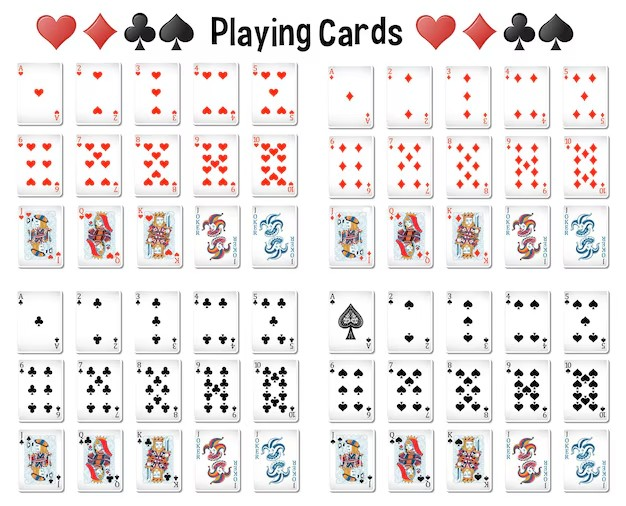
\includegraphics[width=0.72\textwidth]{kartu-remi-lengkap.jpg}\\[2pt]
{\small\textit{Bagan lengkap: $4$ jenis $\times$ $13$ nilai ($\mathrm{A}$--$\mathrm{K}$);
hati \& wajik merah, sekop \& keriting hitam. Permainan NCSC memakai $52$ kartu
ini; \emph{kartu joker tidak disertakan}.}}
\end{center}
\end{berkas}

\medskip

% ---------------------------- NOMOR 6 ----------------------------
\begin{soal}{6}
Gunakan \textbf{Berkas C}.
\begin{subsoal}
  \item Pada tiap ronde, $3$ kartu dibuka satu per satu (\emph{berurutan}, tanpa
        pengembalian). Tentukan banyak susunan berurutan $3$ kartu yang mungkin,
        lalu nyatakan dalam notasi $\,_{52}P_{3}$.
  \item Jika \emph{urutan tidak diperhatikan}, tentukan banyaknya cara memilih $3$
        kartu berbeda, lalu nyatakan dalam notasi $\,_{52}C_{3}$. Jelaskan
        hubungannya dengan hasil (a).
  \item Setiap pemain menerima \textbf{tangan $5$ kartu}. Tentukan banyak tangan
        $5$ kartu berbeda yang mungkin.
  \item Tentukan banyak tangan $5$ kartu yang \textbf{seluruhnya kartu hati}
        ($\heartsuit$).
\end{subsoal}
\end{soal}

% ---------------------------- NOMOR 7 ----------------------------
\begin{soal}{7}
Sebuah kartu diambil \textbf{acak} dari set $52$ kartu (Berkas C), kecuali pada (e).
\begin{subsoal}
  \item Tentukan banyak anggota ruang sampel $n(S)$.
  \item Tentukan peluang terambil kartu \textbf{As}.
  \item Tentukan peluang terambil kartu \textbf{merah}.
  \item Tentukan peluang terambil kartu \textbf{bergambar} ($\mathrm{J}$,
        $\mathrm{Q}$, atau $\mathrm{K}$).
  \item Seorang pemain menerima \textbf{tangan $5$ kartu}. Dengan memakai hasil
        \textbf{Nomor 6(c) dan 6(d)}, tentukan peluang tangan itu \textbf{seluruhnya
        hati} ($\heartsuit$). (Nyatakan sebagai pecahan dan hampiran desimal.)
\end{subsoal}
\end{soal}

% ---------------------------- NOMOR 8 ----------------------------
\begin{soal}{8}
Sepanjang turnamen tercatat \textbf{$1.300$ kali pengambilan kartu} (tiap kali
dikembalikan lalu dikocok ulang, sehingga peluang tiap kejadian tetap).
\begin{subsoal}
  \item Tentukan frekuensi harapan munculnya kartu \textbf{As}.
  \item Tentukan frekuensi harapan munculnya kartu \textbf{merah}.
  \item Tentukan frekuensi harapan munculnya kartu \textbf{bergambar}.
  \item Tentukan frekuensi harapan munculnya \textbf{As sekop} ($\mathrm{A}\spadesuit$)
        secara spesifik.
  \item Pengamatan nyata mencatat As muncul \textbf{$92$ kali}. Hitung selisihnya
        terhadap frekuensi harapan (a), nyatakan selisih itu sebagai
        \textbf{persentase} dari frekuensi harapan, lalu simpulkan: tergolong
        \emph{selisih kecil} (di bawah $10\%$) atau \emph{selisih besar} ($\ge10\%$)?
\end{subsoal}
\end{soal}

% ---------------------------- NOMOR 9 ----------------------------
\begin{soal}{9}
Gunakan \textbf{Berkas C}. Satu kartu diambil \textbf{acak}, kecuali disebutkan lain.
\begin{subsoal}
  \item Tentukan peluang kartu yang terambil \textbf{bukan As}.
  \item Tentukan peluang terambil kartu \textbf{As atau King}.
  \item Tentukan peluang terambil kartu \textbf{As atau merah}.
  \item Dua kartu diambil satu per satu \textbf{dengan pengembalian}. Tentukan
        peluang \textbf{keduanya merah}.
  \item Dua kartu diambil \textbf{tanpa pengembalian}. Tentukan peluang
        \textbf{keduanya merah}, lalu bandingkan dengan hasil (d) dan jelaskan
        mengapa berbeda.
\end{subsoal}
\end{soal}

\clearpage
\noindent{\large\bfseries BAGIAN C: Sintesis Statistika--Peluang (Nomor 10)}\\[0.2em]
\small\emph{Kini seluruh berkas terbuka. Satukan temuan Bagian A--B untuk keputusan
akhir panitia --- termasuk \textbf{menindaklanjuti pencilan yang Anda temukan di
Nomor 5}. Kenali sendiri konsep yang diperlukan tiap bagian; tutup dengan simpulan
seorang analis.}\normalsize

\bigskip

% ---------------------------- NOMOR 10 ----------------------------
\begin{soal}{10}
Gunakan \textbf{Berkas A} (skor $40$ peserta), \textbf{Berkas B} (Nomor 5), dan
\textbf{Berkas C} (set remi). Seorang \emph{peserta} dipilih \textbf{acak}, kecuali
disebutkan lain.
\begin{subsoal}
  \item \textbf{(Peluang dari sebaran.)} Tentukan peluang skor peserta berada pada
        kelas $20$--$29$, dan peluang skornya \textbf{kurang dari $20$}.
  \item \textbf{(Mengapa kuartil?)} Gelar \textbf{``peserta unggulan''} diberikan
        kepada $25\%$ peserta ber-poin minus terkecil, yaitu yang berada di bawah
        $Q_1=15{,}5$ (Nomor 3). \textbf{(i)} \emph{Tanpa} menghitung ulang frekuensi,
        jelaskan mengapa peluang seorang peserta acak bergelar unggulan \emph{pasti}
        sama dengan $25\%$. \textbf{(ii)} Rata-rata skor $=25$, padahal $Q_1=15{,}5$.
        Jelaskan mengapa panitia memakai \emph{kuartil}, bukan \emph{rata-rata},
        sebagai ambang gelar (kaitkan dengan sebaran condong kanan pada Nomor 2).
  \item \textbf{(Frekuensi harapan \& gabungan.)} Musim depan $200$ peserta,
        distribusi sama. \textbf{(i)} Tentukan frekuensi harapan peserta unggulan.
        \textbf{(ii)} Dua peserta dipilih \textbf{tanpa pengembalian}; tentukan
        peluang \textbf{keduanya unggulan}. \textbf{(iii)} Untuk undian hadiah,
        dipilih satu peserta acak \emph{dan} ditarik satu kartu remi; bila kejadian
        ``peserta unggulan'' dan ``kartu As'' \textbf{bebas}, tentukan peluang
        keduanya terjadi.
  \item \textbf{(Tindak lanjut pencilan.)} Ingat temuan Nomor 5: \textbf{Bima}
        adalah pencilan (berpikir lama, tetapi poin minus tetap tinggi).
        \textbf{(i)} Apakah satu pencilan seperti Bima \emph{membatalkan} kesimpulan
        ``hasil ditentukan keterampilan''? Jelaskan. \textbf{(ii)} Jika data Bima
        dikeluarkan, apakah korelasi waktu--skor \emph{menguat} atau \emph{melemah}?
        Mengapa?
  \item \textbf{(Rekomendasi.)} Panitia menyebut sistem \textbf{adil dan seimbang}
        bila: \textbf{(I)} frekuensi kemunculan kartu mendekati peluang teoretisnya,
        \textbf{dan (II)} sebaran skor terkendali serta hasil condong ke keterampilan.
        Nilailah sistem NCSC dengan kedua indikator itu: dukung dengan \textbf{minimal
        dua hasil statistik} (Nomor 2--5) dan \textbf{minimal satu hasil peluang}
        (Nomor 7--9), lalu beri \textbf{satu saran perbaikan}.
\end{subsoal}
\end{soal}

\clearpage
\noindent{\large\bfseries BAGIAN D: Soal Bonus (Nomor 11--12)}\\[0.2em]
\small\emph{Kerjakan hanya bila Nomor 1--10 selesai. Benar menambah poin;
salah/kosong tidak mengurangi.}\normalsize

\bigskip

% ---------------------------- NOMOR 11 (BONUS) ----------------------------
\begin{soal}{11 \normalfont\bfseries[BONUS]}
\begin{berkas}{Berkas D: Sepuluh Kartu Penentu Kemenangan}
\centering\small
Setiap kartu dalam set diberi \textbf{nomor urut $1$--$52$}. Sepanjang turnamen,
panitia mendata \textbf{sepuluh nomor kartu yang paling sering menjadi penentu
kemenangan} di meja-meja final (tercatat pada lembar rekap, gambar pembuka):
\[
2,\quad 4,\quad 8,\quad 14,\quad 19,\quad 23,\quad 24,\quad 31,\quad 38,\quad 44.
\]
(Data \emph{tunggal/tidak dikelompokkan}, sudah terurut naik; semuanya $\le52$.)
\end{berkas}

\smallskip
Sebagai analis, ringkas sebaran sepuluh nomor kartu penentu itu sebagai data tunggal.
\begin{subsoal}
  \item Tentukan rata-rata (mean).
  \item Tentukan median dan modus.
  \item Tentukan kuartil bawah $Q_1$, kuartil atas $Q_3$, dan jangkauan
        antarkuartil (gunakan metode membagi data menjadi dua bagian).
  \item Tentukan jangkauan (\emph{range}) dan beri satu kalimat interpretasi
        tentang sebaran nomor kartu penentu.
\end{subsoal}
\end{soal}

% ---------------------------- NOMOR 12 (BONUS) ----------------------------
\begin{soal}{12 \normalfont\bfseries[BONUS]}
Panitia ingin memastikan bahwa munculnya kartu istimewa tidak ``terlalu mudah''.
Gunakan Berkas C dan nilai bantu pada petunjuk.
\begin{subsoal}
  \item Dua kartu diambil tanpa pengembalian. Tentukan peluang keduanya
        \textbf{berpasangan} (bernilai/rank sama, misalnya dua-duanya $7$).
  \item Tentukan peluang sebuah tangan $5$ kartu berisi \textbf{tepat dua As}.
        (Gunakan $\binom{4}{2}$, $\binom{48}{3}$, dan $\binom{52}{5}$.)
  \item Berdasarkan (b), jelaskan secara singkat: jika sistem adil, mengapa
        memperoleh ``tepat dua As'' tergolong \emph{jarang}, dan apa artinya bagi
        keseimbangan permainan?
\end{subsoal}
\end{soal}
\end{document}

